\PassOptionsToPackage{unicode}{hyperref}
\documentclass[aspectratio=1610, 9pt]{beamer}

% Load packages you need here
\usepackage{polyglossia}
\setmainlanguage{german}

\usepackage{csquotes}
\usepackage{graphicx}
\usepackage{siunitx}
\usepackage{amsmath}
\usepackage{amssymb}
\usepackage{mathtools}

\usepackage{hyperref}
\usepackage{bookmark}

% load the theme after all packages

\usetheme[
  %showtotalframes, % show total number of frames in the footline
   % dark, % optional dark theme, uncomment to use
]{tudo}

% Put settings here, like
\unimathsetup{
  math-style=ISO,
  bold-style=ISO,
  nabla=upright,
  partial=upright,
  mathrm=sym,
}
\begin{document}
\title{Observing the Prompt Component of the Atmospheric Muon Flux Using IceCube}
\date{3 April 2025}
\author{Leander Flottau}
%\institute{Astroteilchenphysik \\  Fakultät: Physik}
\titlegraphic{
\includegraphics[width=0.7\textwidth]{Plots/IceCube_webheader_fullcolor}}
\begin{document}
\maketitle
%\begin{frame}
%  \frametitle{Table of Contents}
%  \tableofcontents
%\end{frame}  
%\section{IceCube Neutrino Observatory}
\begin{frame}
    \frametitle{IceCube Neutrino Observatory}
    \begin{minipage}{0.6\textwidth}
        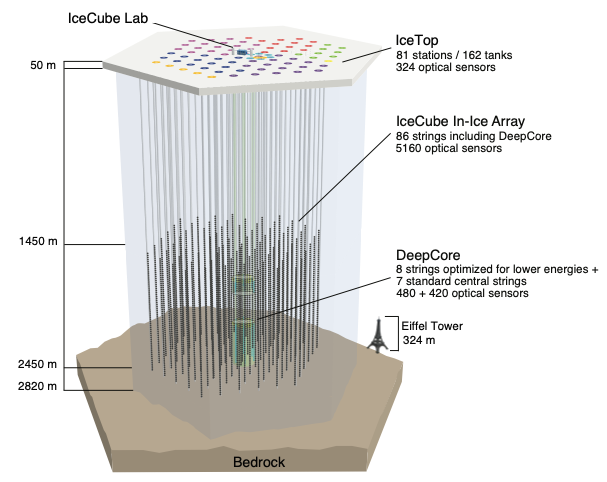
\includegraphics[width=\textwidth]{Plots/IceCube schematic}
    \end{minipage}
    \begin{minipage}{0.39\textwidth}
        \begin{itemize}
            \item Cubic kilometer scale cherenkov detector
            \item $5160$ DOMs on $86$ strings
            %\item ~$270$ measured neutrino Events per day
            \item ~$\approx \SI{3}{\kilo\hertz}$ muon event rate
        \end{itemize}
    \end{minipage}
\end{frame}
\begin{frame}
    \frametitle{Atmospheric Air Showers}
%    \begin{minipage}{0.6\textwidth}
    \begin{figure}
        \centering
        \includegraphics[width=0.6\textwidth]{Plots/Air Shower Illustration}
    \end{figure}
%    \end{minipage}
%    \begin{minipage}{0.39\textwidth}
%        \begin{itemize}
%            \item Cosmic ray interactions produce secondary particles
%            \item Major decay product: $\mu$
%        \end{itemize}
%    \end{minipage}
\end{frame}
\begin{frame}
    \frametitle{The Prompt Component}
    \begin{minipage}{0.6\textwidth}
        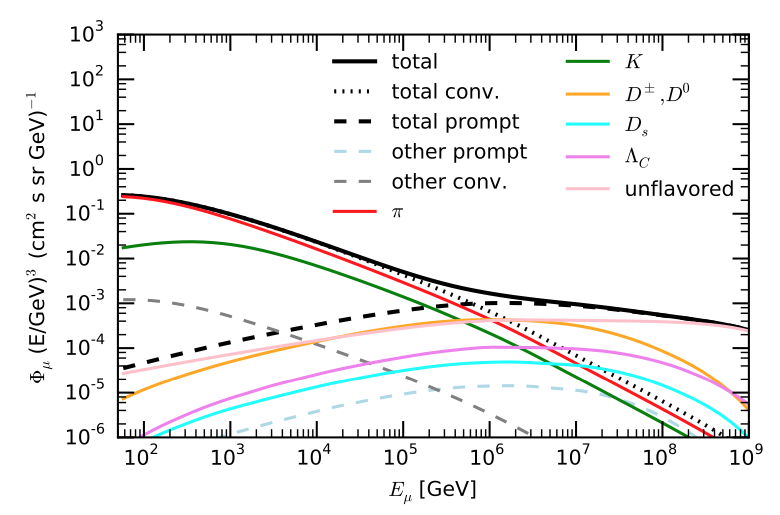
\includegraphics[width=0.75\textwidth]{Plots/Prompt vs conventional flux}
    \end{minipage}
    \begin{minipage}{0.39\textwidth}
        \begin{itemize}
            \item Conventional: produced by $K^{\pm}$/$\pi^{\pm}$
            \item Prompt: produced by short-lived particles
            \item Prompt dominant at high energies
        \end{itemize}
    \end{minipage}
\end{frame}
\begin{frame}
    \frametitle{Prompt sensitivity}
    \begin{minipage}{0.6\textwidth}
        \begin{figure}
            \centering
            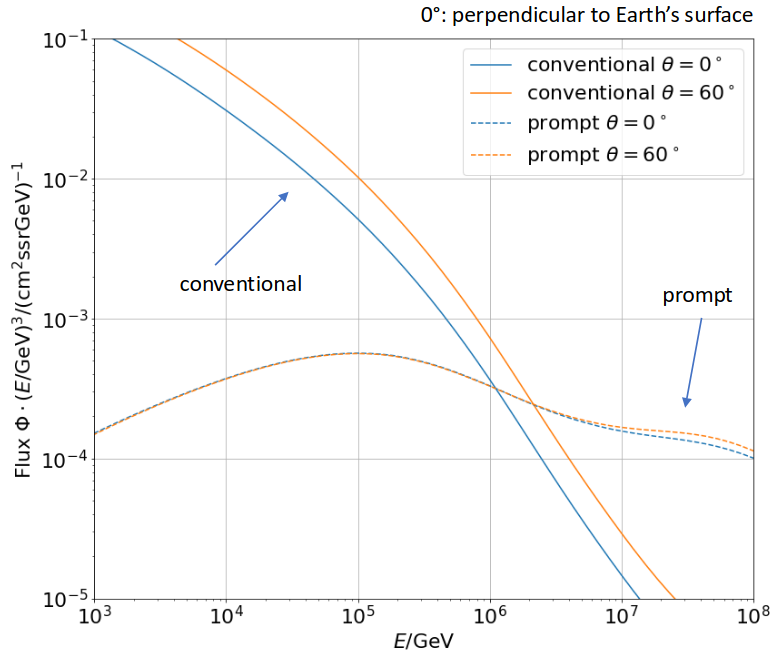
\includegraphics[width=\textwidth]{Plots/prompt_flux_zenith}
        \end{figure}
    \end{minipage}
    \begin{minipage}{0.39\textwidth}
        \begin{itemize}
            \item Sensitivity increases at high energies
            \item Prompt less impacted by the zenith angle
        \end{itemize}
    \end{minipage}
\end{frame}
\begin{frame}
    \frametitle{The Muon-Puzzle}
    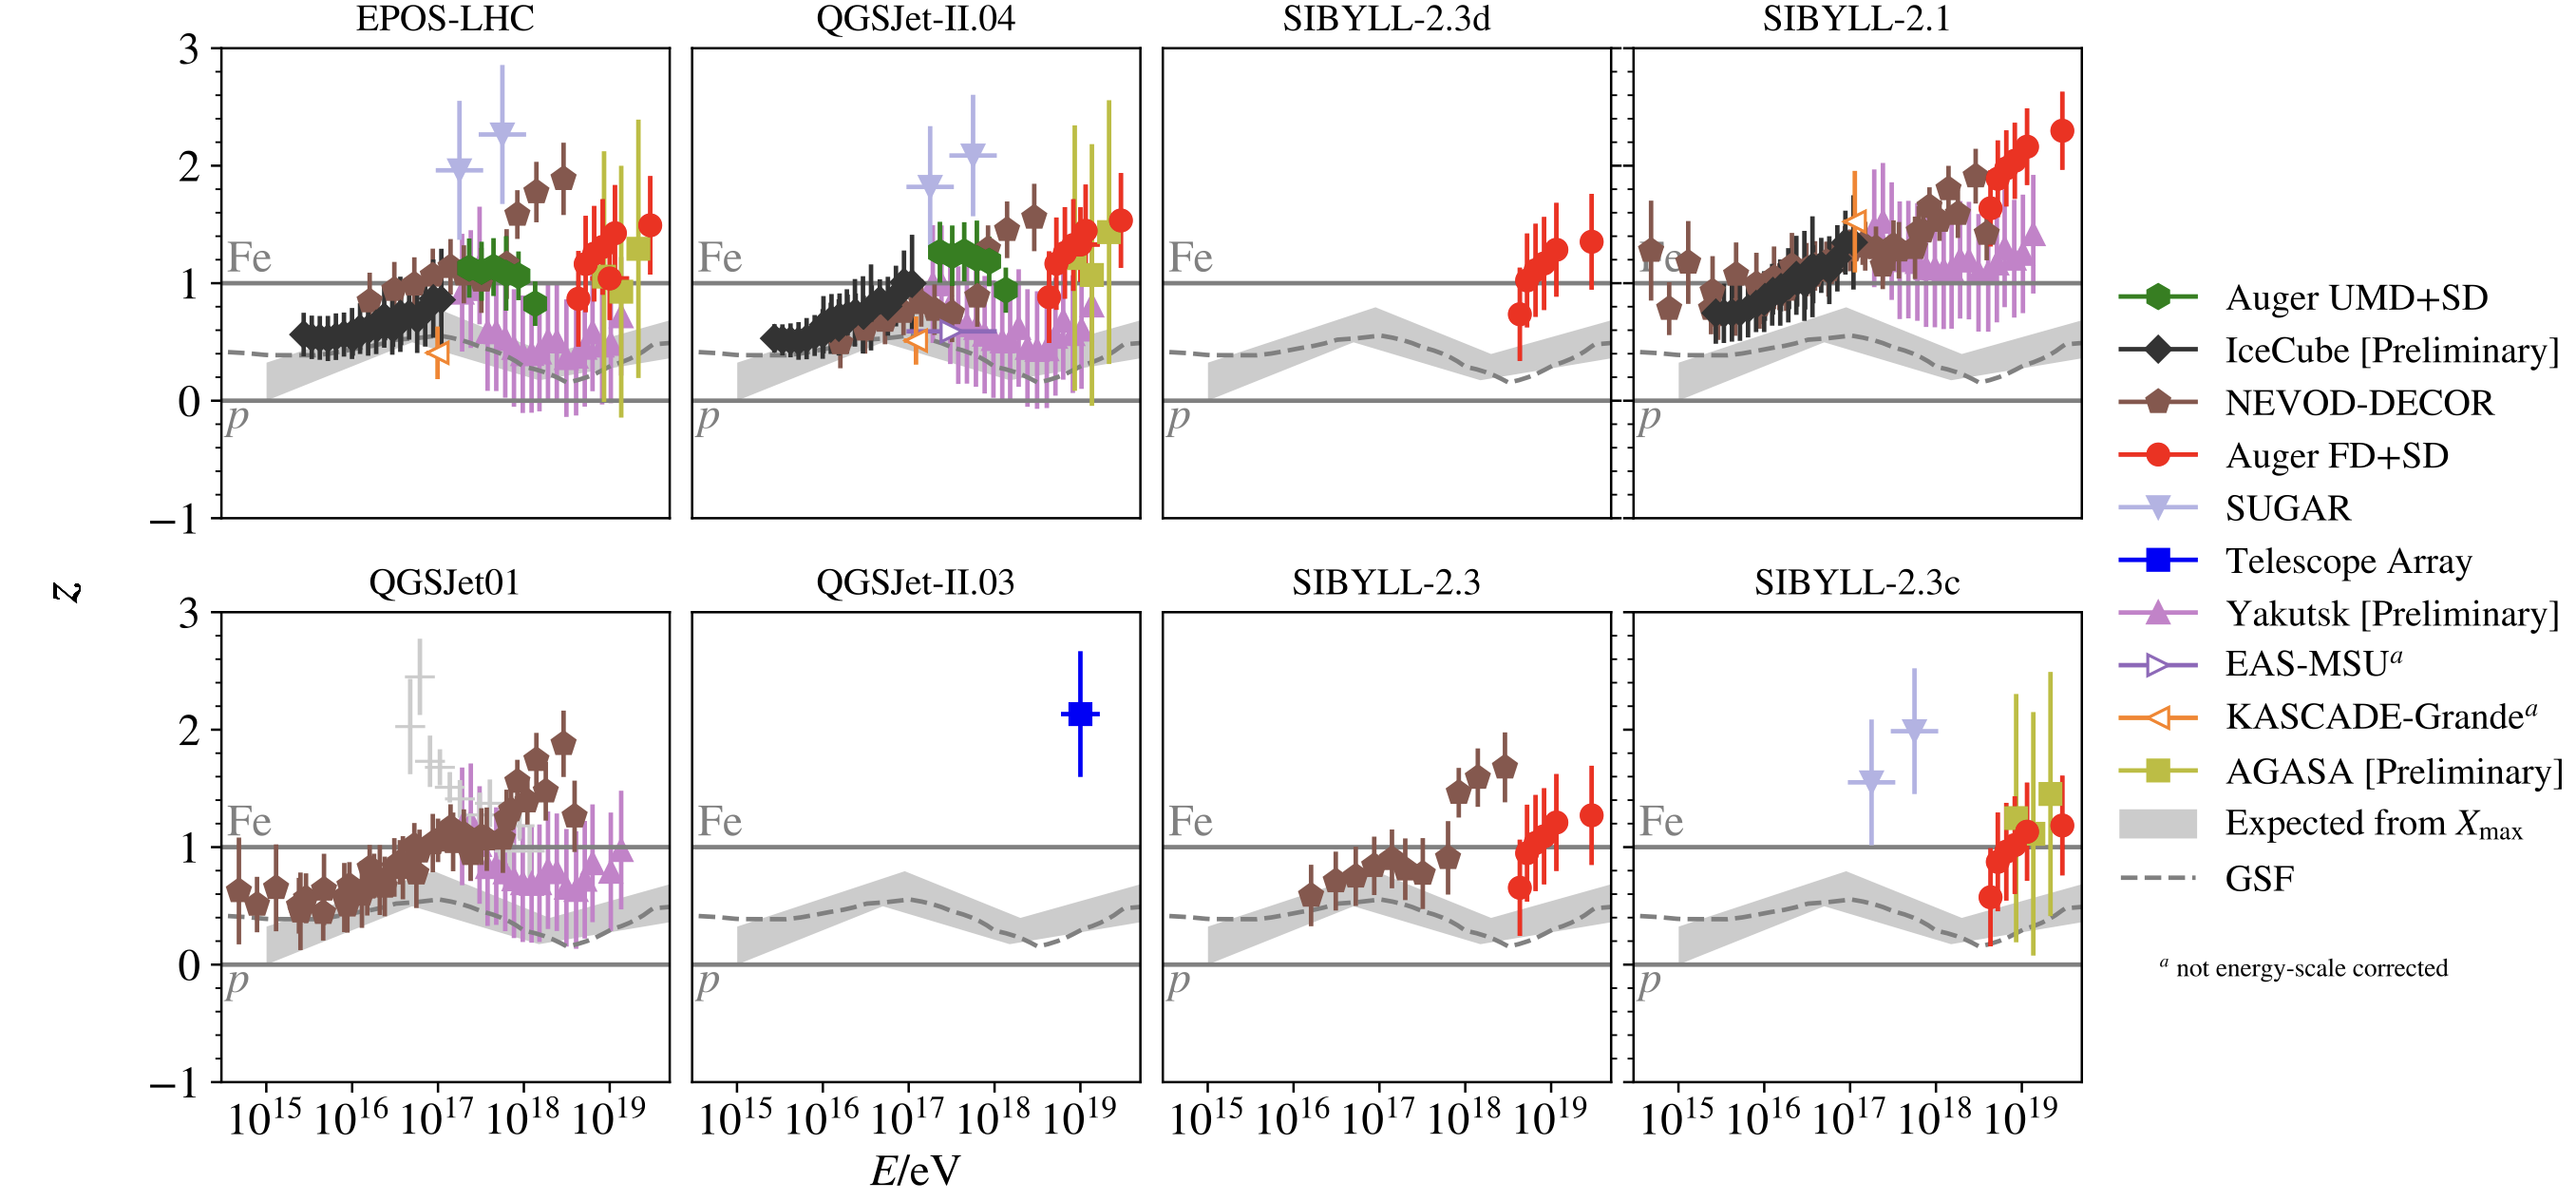
\includegraphics[width=0.9\textwidth]{Plots/muon puzzle}
%    \begin{itemize}
%        \item More muons measured than simulations predicted
%        \item Hadronic interaction models
%    \end{itemize}
\end{frame}
\begin{frame}
    \frametitle{Simulations and tagging}
    \begin{minipage}{0.5\textwidth}
        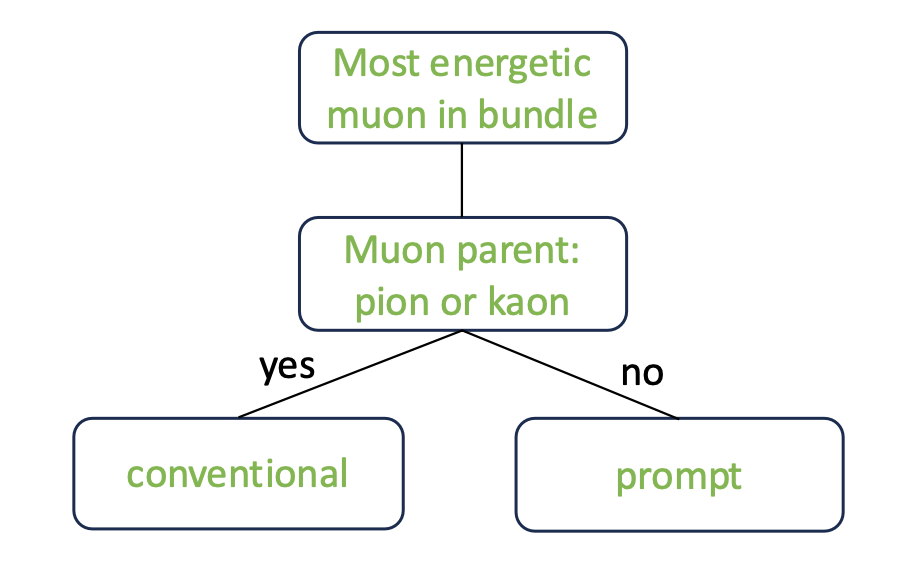
\includegraphics[width=0.8\textwidth]{Plots/prompt_tagging}
    \end{minipage}
    \begin{minipage}{0.49\textwidth}
        \begin{itemize}
            \item Tagging of parent particles in CORSIKA simulations
            \item Prompt definition based on parent of leading muon
%        \item Allows for MC-Sample with prompt/conventional distinction 
            \item Simulation up to extremely high energies
        \end{itemize}
    \end{minipage}
\end{frame}
\begin{frame}
    \frametitle{Reconstructions}
    \begin{minipage}{0.6\textwidth}
        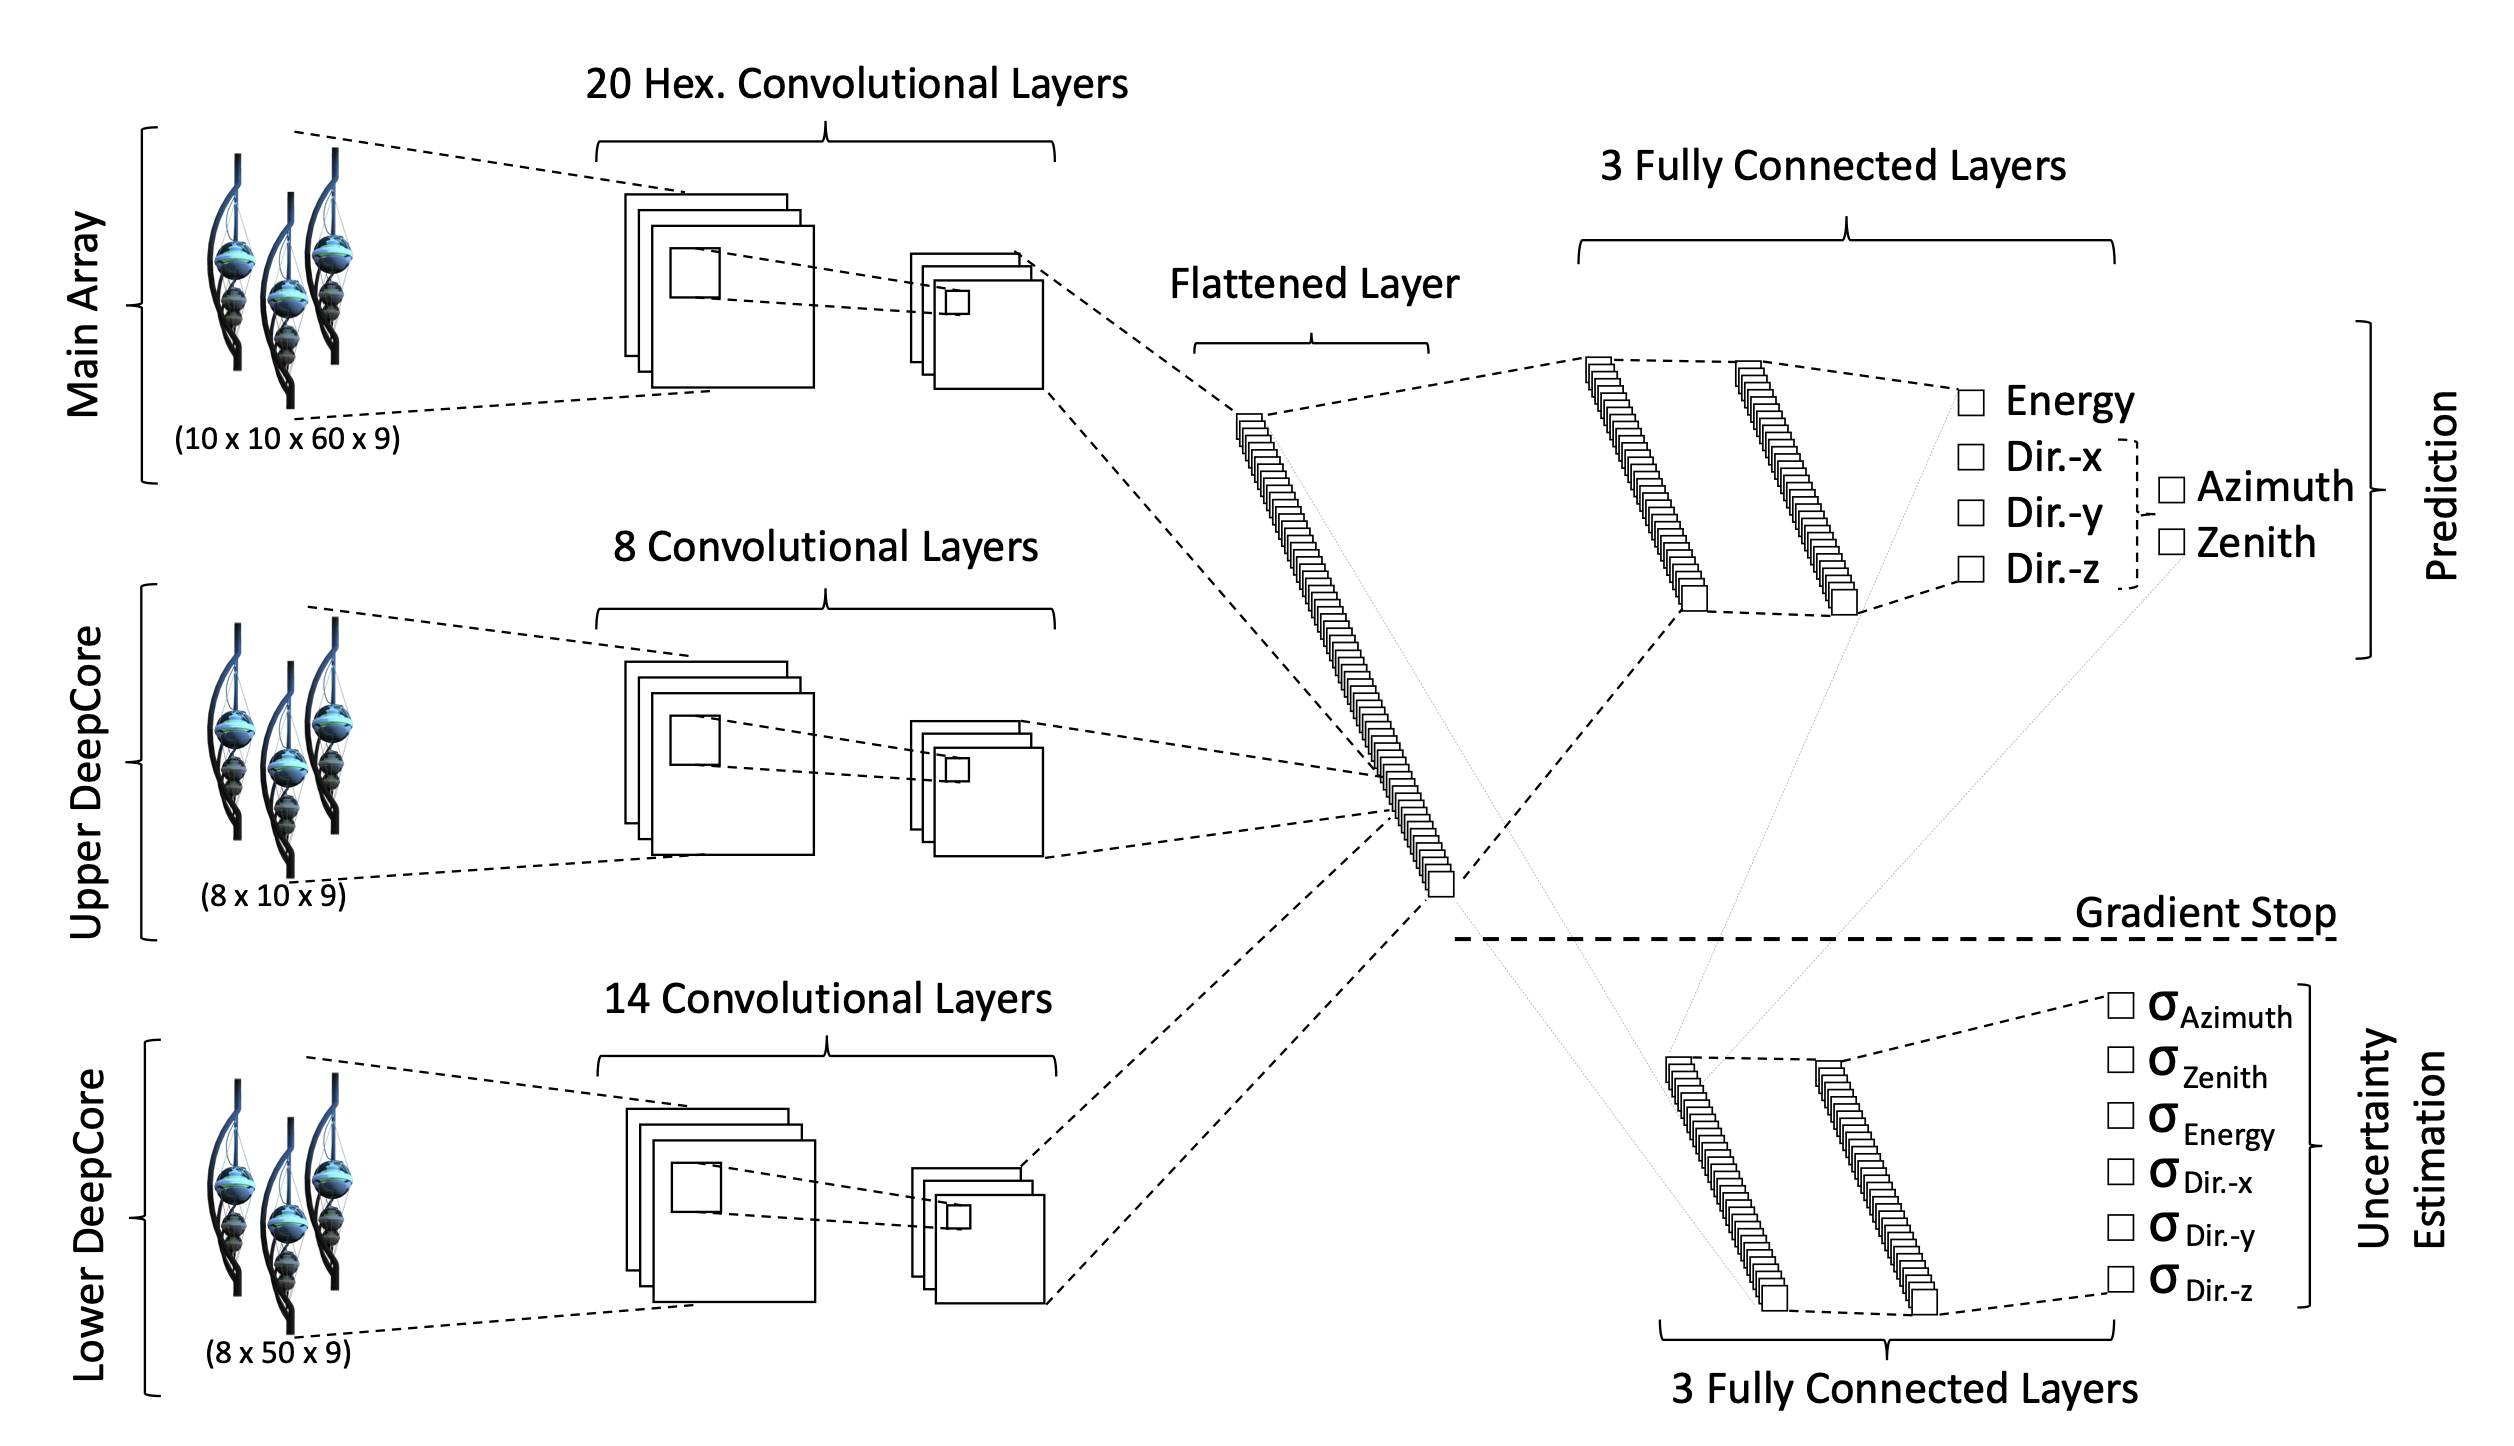
\includegraphics[width=\textwidth]{Plots/DNN_architecture}
    \end{minipage}
    \begin{minipage}{0.39\textwidth}
        \begin{itemize}
            \item Neural network based
            \item Zenith angle, bundle energy and leading muon energy
        \end{itemize}
    \end{minipage}
\end{frame}
\begin{frame}
	\frametitle{Reconstructions}
    \begin{figure}
        \centering
        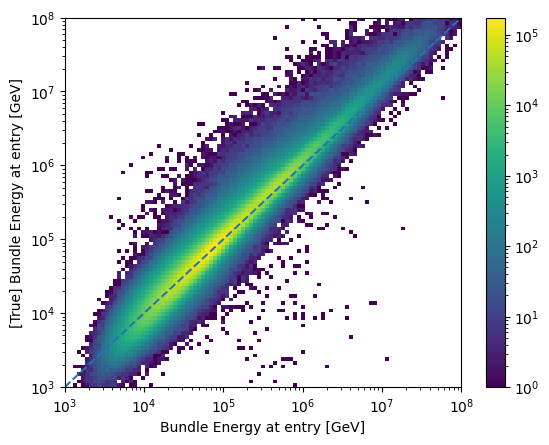
\includegraphics[width=0.49\textwidth]{Plots/bundle_correlation_colorbar}
        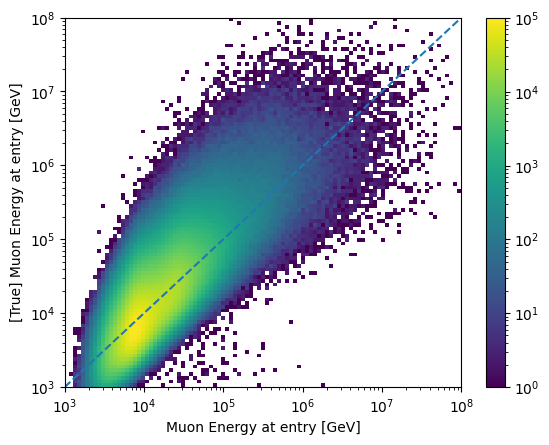
\includegraphics[width=0.49\textwidth]{Plots/entry_correlation_colorbar}
    \end{figure}
\end{frame}
\begin{frame}
    \frametitle{Forward Folding}
    \begin{minipage}{0.6\textwidth}
        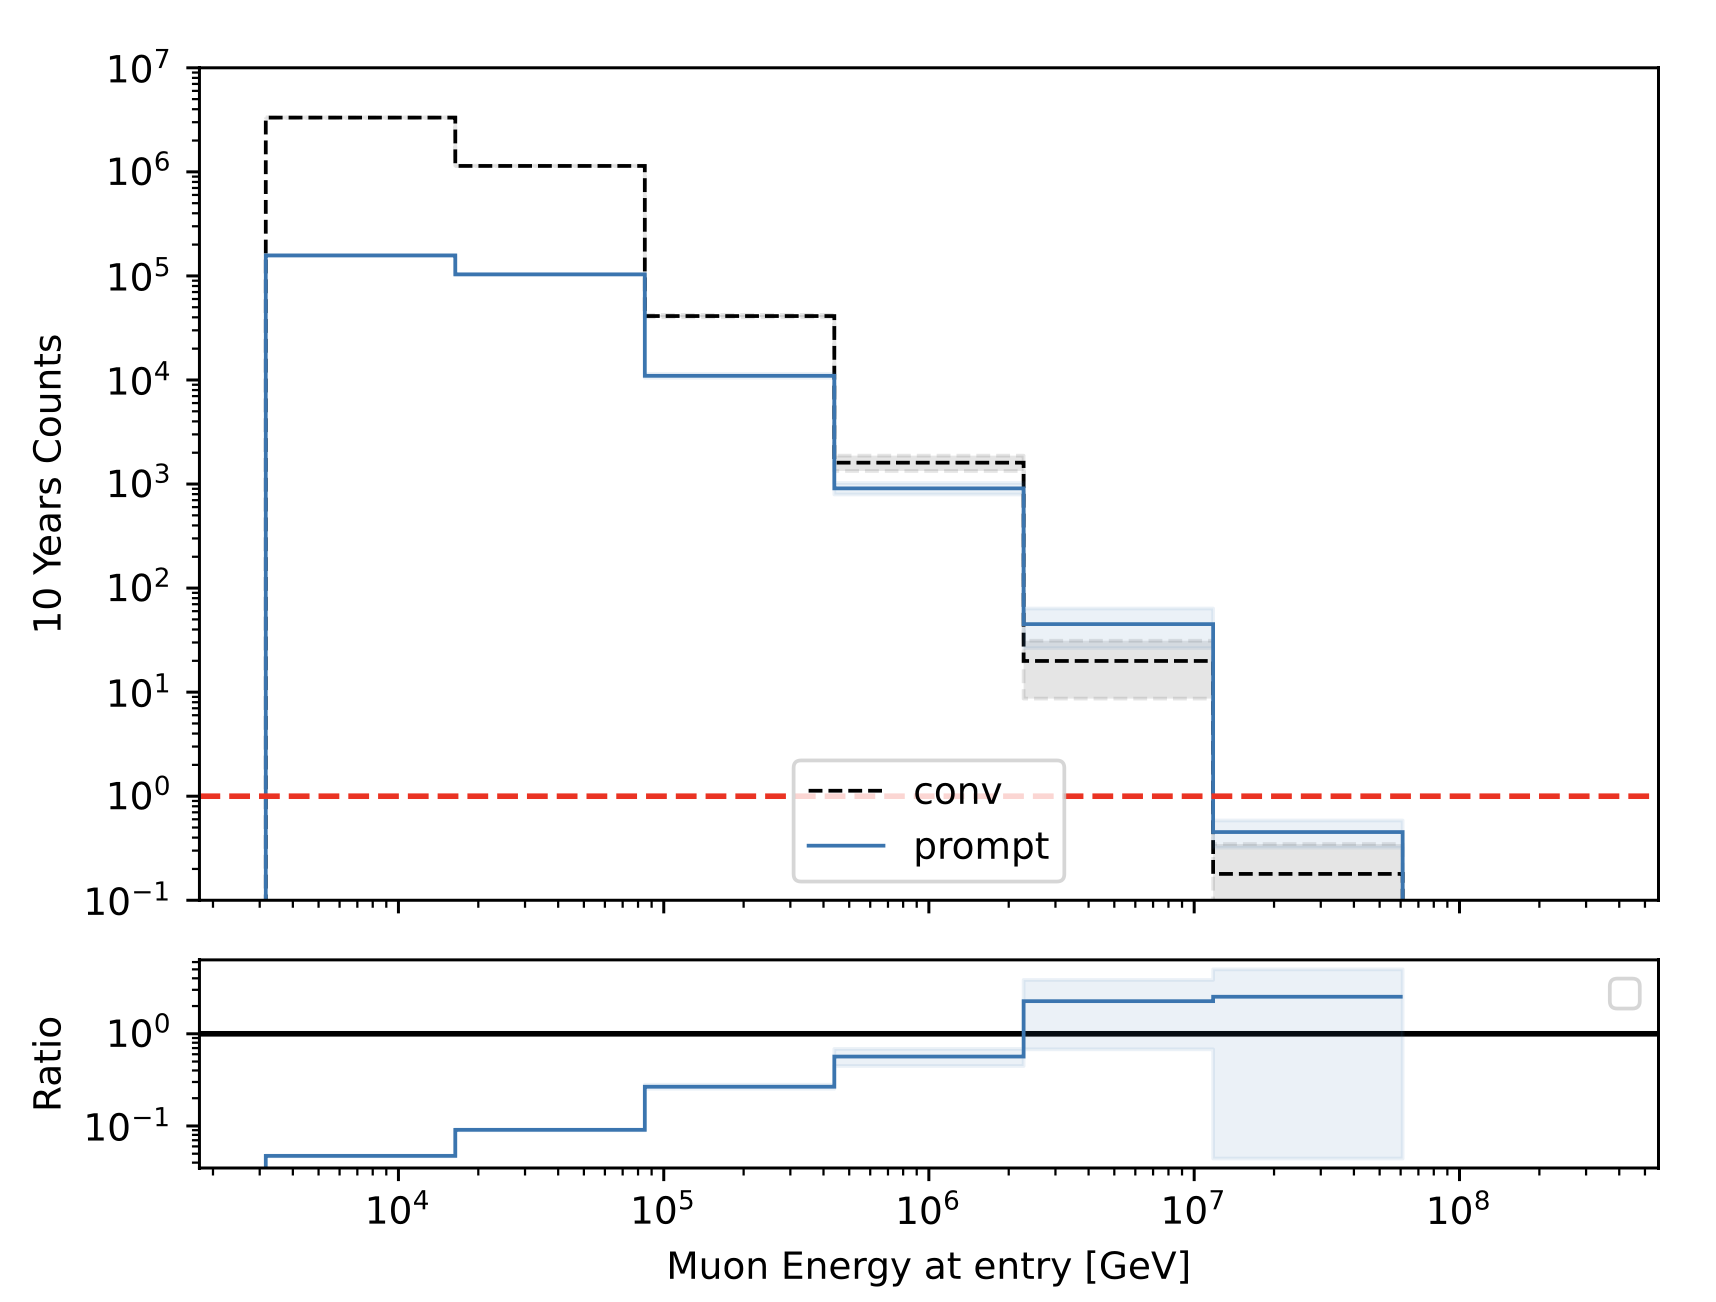
\includegraphics[width=\textwidth]{Plots/spectrum_(3.5,8.5,8)_10Y.png}
    \end{minipage}
    \begin{minipage}{0.39\textwidth}
        \begin{itemize}
            \item Prompt normalization: fraction of prompt component relative to current MC-simulation $n_{pr}$
            \item Poisson likelihood in each histogram bin
            \item Rescale with normalization factors 
            \item Strong model dependency
        \end{itemize}
    \end{minipage}
\end{frame}
\begin{frame}
    \frametitle{Pseudo experiments and asimov tests}
    \begin{minipage}{0.6\textwidth}
        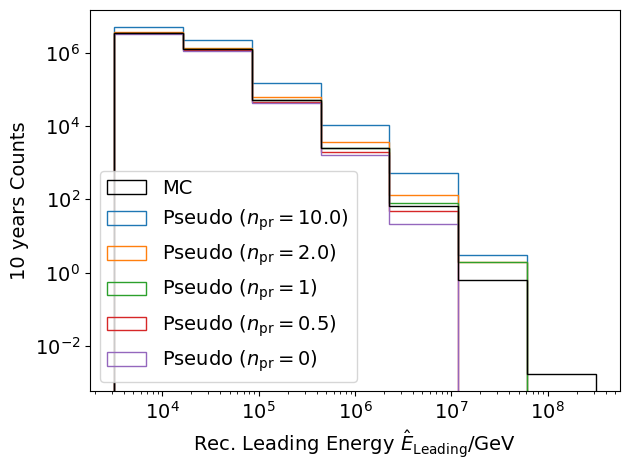
\includegraphics[width=\textwidth]{Plots/injected norms.png}
    \end{minipage}
    \begin{minipage}{0.39\textwidth}
        \begin{itemize}
            \item Testing method based on simulations
            \item Asimov: Toy data resembling the MC expectation given the injected input parameters
            \item Pseudoexperiments: Sampled based on weights
        \end{itemize}
    \end{minipage}
\end{frame}
\begin{frame}
    \frametitle{Background Estimation}
    \begin{minipage}{0.6\textwidth}
        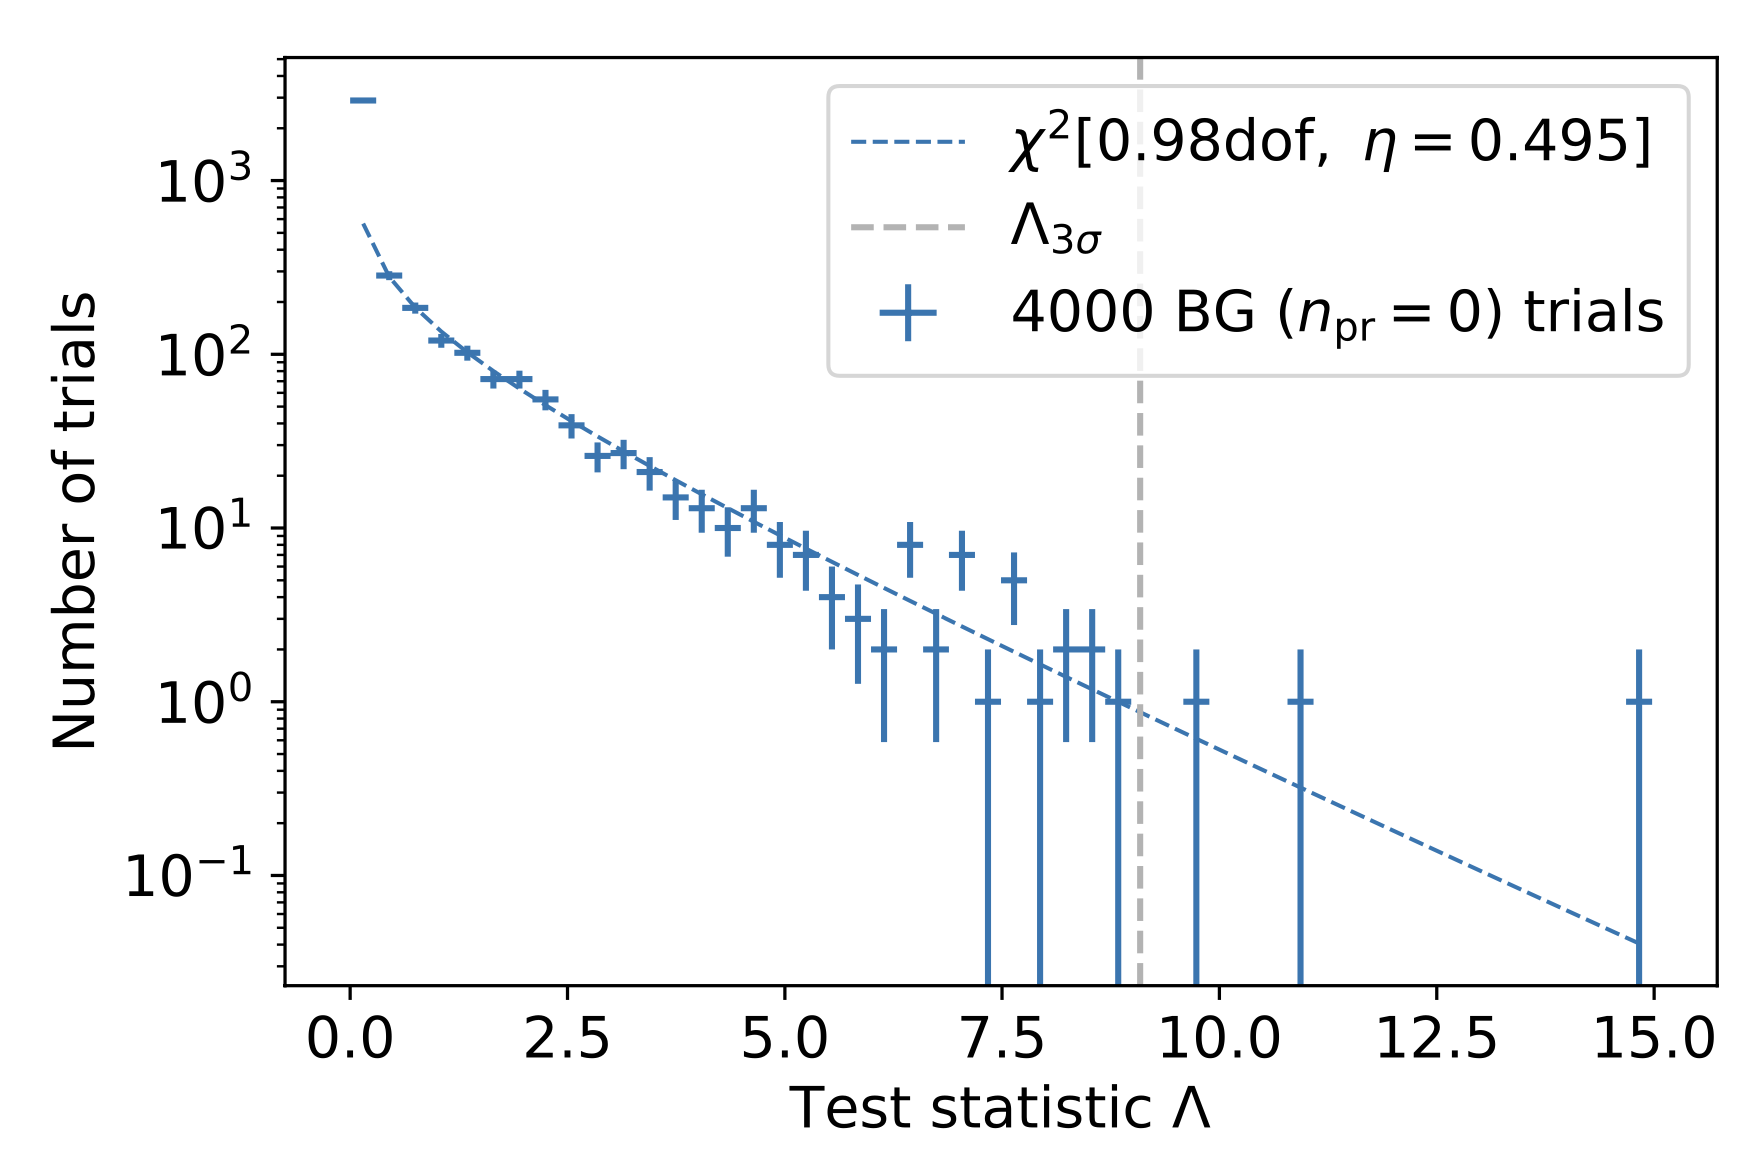
\includegraphics[width=\textwidth]{Plots/background_statistic_chi2_(3.5,8.5,8)_10Yp.png}
    \end{minipage}
    \begin{minipage}{0.39\textwidth}
        \begin{itemize}
            \item Likelihood ratio test: $\lambda = -2(llh(\Theta_0)-llh(\Theta))$
            \item Draw background samples with $n_{pr}=0$
            \item Wilks' theorem: fit $\Chi^2$-distribution
        \end{itemize}
    \end{minipage}
\end{frame}
%\begin{frame}
%    \frametitle{Discovery Potential: First Estimate}
%    \begin{minipage}{0.6\textwidth}
%        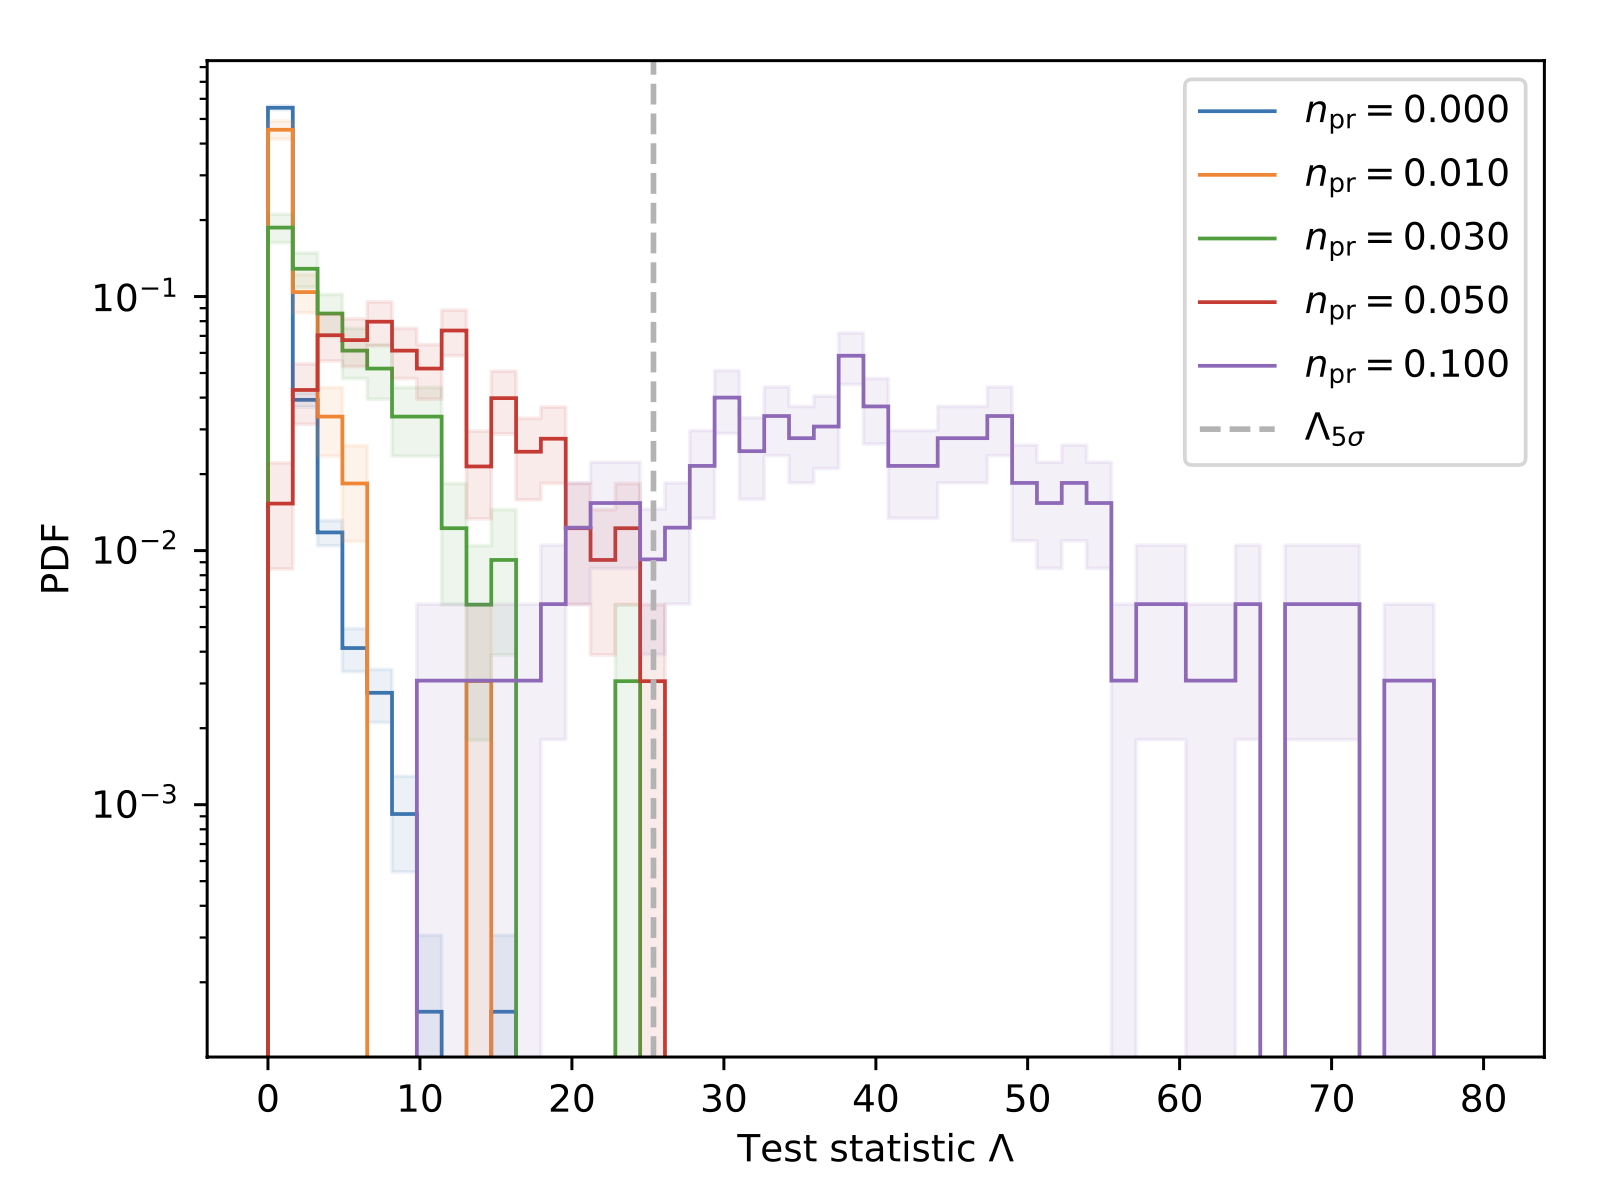
\includegraphics[width=\textwidth]{Plots/TS_Distribution(3.5,8.5,8)_10Y.png}
%    \end{minipage}
%    \begin{minipage}{0.39\textwidth}
%        \begin{itemize}
%            \item Prompt norm required to detect it with the current method?
%            \item Discovery potential: Norm at which half the generated trials yield $5 \sigma$ significance in the likelihood ratio test
%            \item Caution: Systematics are not yet included
%	    \item Switch to NNMFit
%        \end{itemize}
%    \end{minipage}
%\end{frame}
\begin{frame}
	\frametitle{Systematic Parameters: SnowStorm}
	\begin{minipage}{0.39\textwidth}
		\begin{itemize}
			\item Detector parameters regarding the ice and DOMs
            \item $5$-Parameters: Absorption, Scattering, DOM-Efficiency, 2 hole-ice models
			\item SnowStorm Ensemble: Individual systematics sampled each event
			\item Drawn from uniform distribution
		\end{itemize}
	\end{minipage}
	\begin{minipage}{0.6\textwidth}
		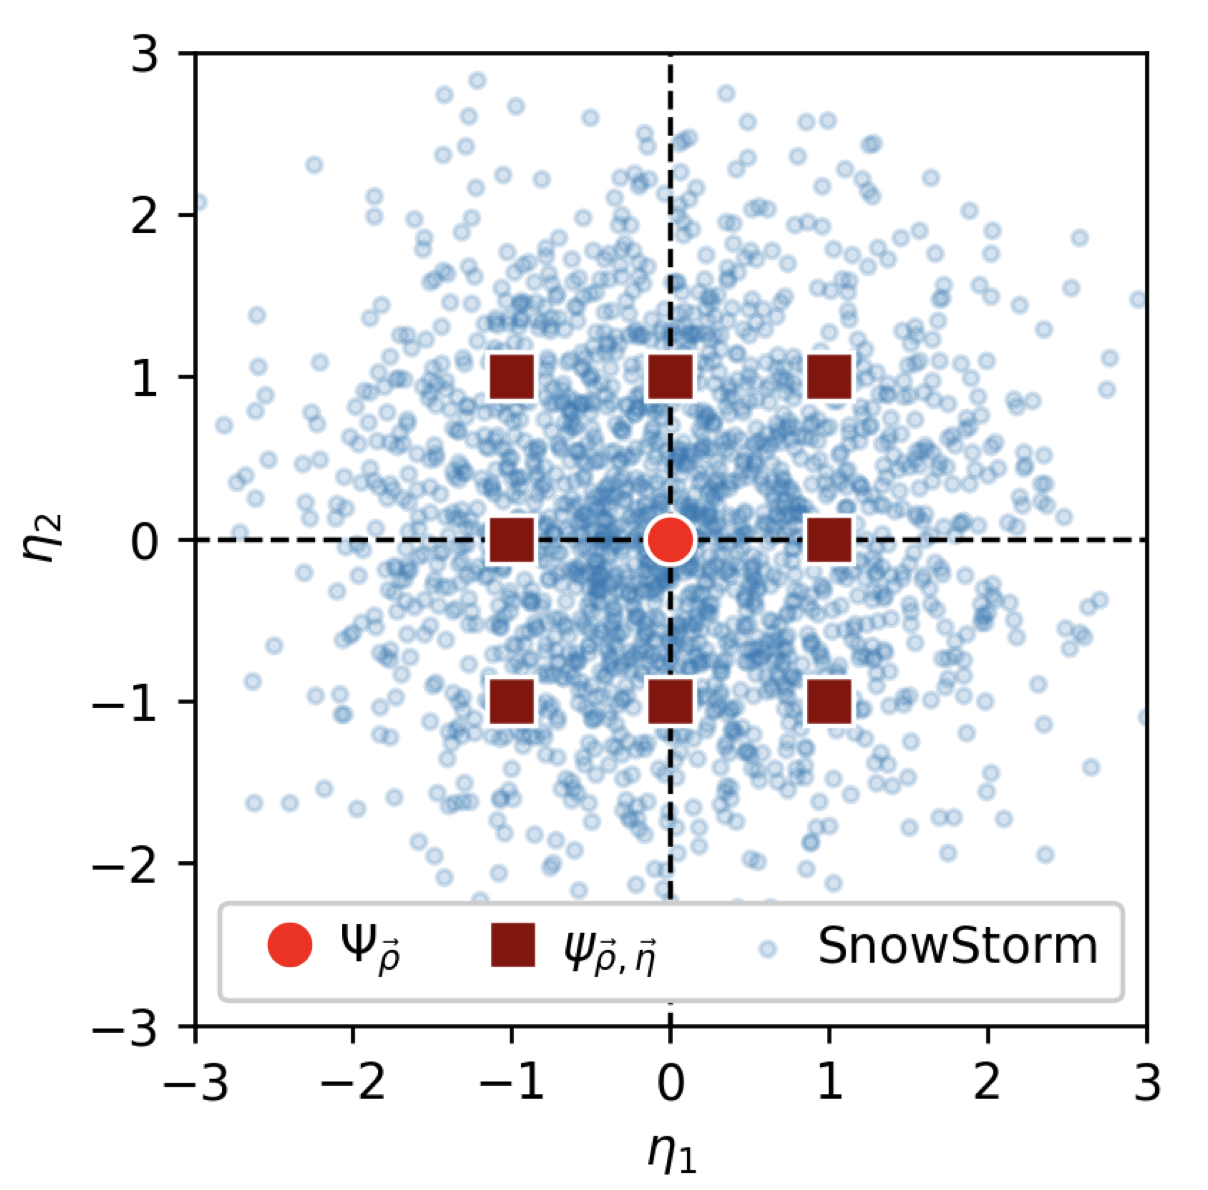
\includegraphics[width=0.8\textwidth]{Plots/SnowStormEnsemble}
	\end{minipage}
\end{frame}
\begin{frame}
	\frametitle{Systematics: Reweighting}
	\begin{minipage}{0.6\textwidth}
		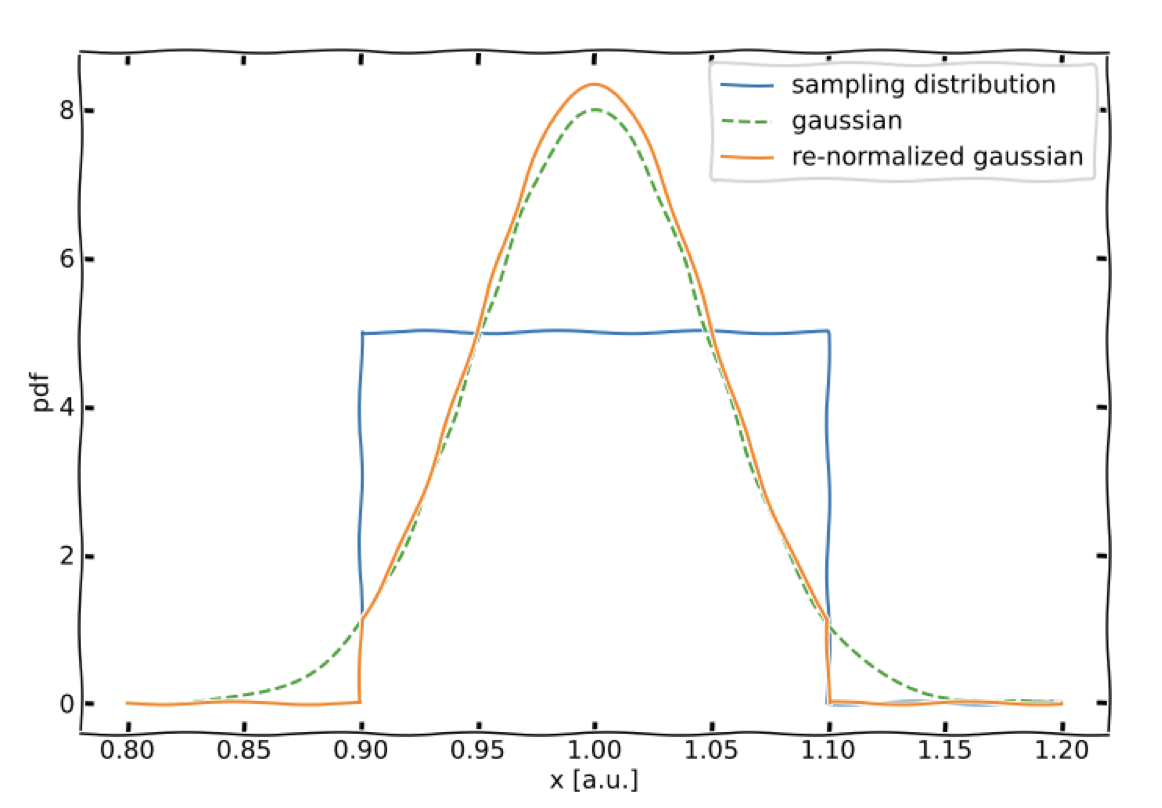
\includegraphics[width=\textwidth]{Plots/SnowStormReweighting}
	\end{minipage}
	\begin{minipage}{0.39\textwidth}
		\begin{itemize}
			\item How do the parameters impact the bincount?
			\item Reweighting
			\item "Inject" hypothesis for parameter by reweighting
            \item Fit mean of reweighting distribution as nuisance parameter
		\end{itemize}
	\end{minipage}
\end{frame}
%\begin{frame}
%	\frametitle{Detector Parameters}
%	\begin{minipage}{0.6\textwidth}
%		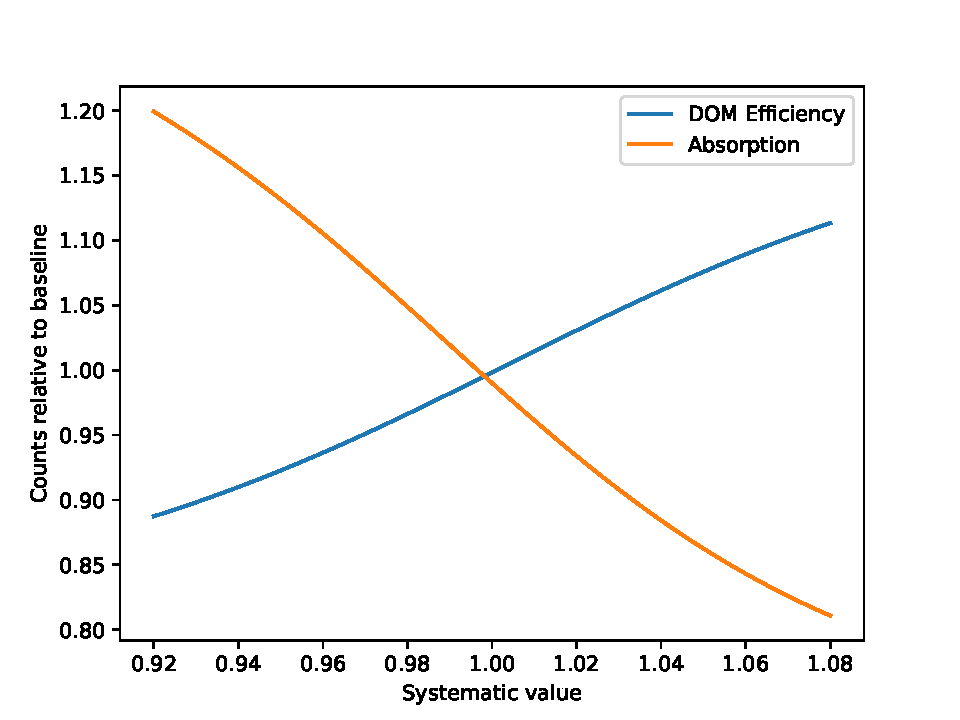
\includegraphics[width=\textwidth]{Plots/SystematicVisualization}
%	\end{minipage}
%	\begin{minipage}{0.39\textwidth}
%		\begin{itemize}
%			\item Simple Visualization of counts in first bin
%            \item Absorption: High absorption shifts events to lower energies
%            \item DOM-Efficiency: High DOM-Efficiency shifts events to higher energies
%		\end{itemize}
%	\end{minipage}
%\end{frame}
\begin{frame}
    \frametitle{Detector Parameters}
    \begin{minipage}{0.6\textwidth}
        \begin{figure}
            \centering
            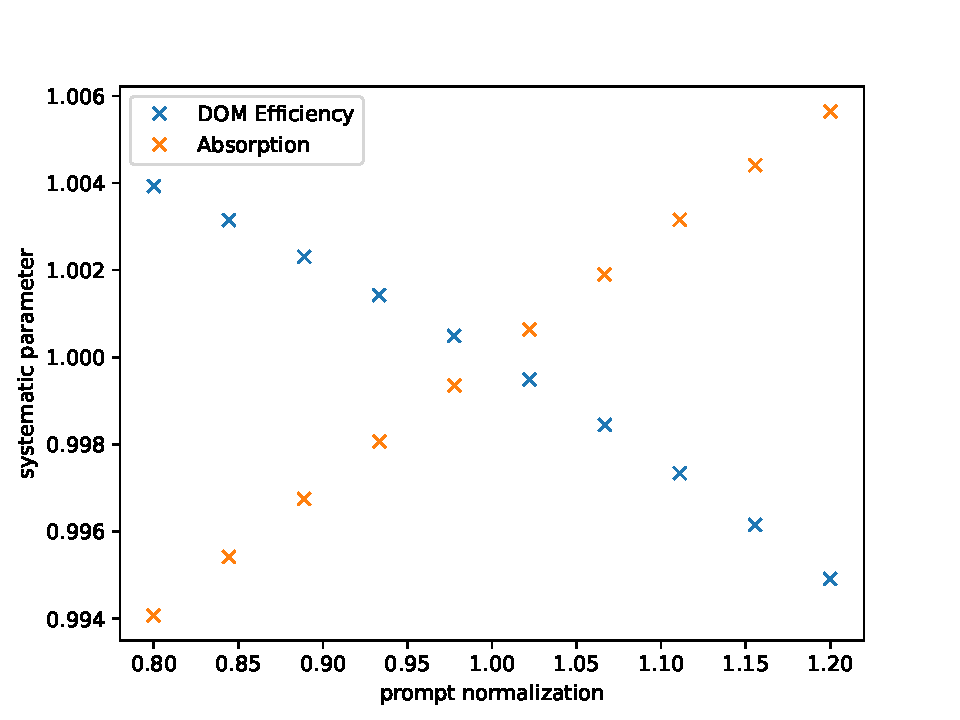
\includegraphics[width=\textwidth]{Plots/systematics_fit_impact}
        \end{figure}
    \end{minipage}
    \begin{minipage}{0.39\textwidth}
        \begin{itemize}
            \item How do these parameters impact the likelihood?
            \item Test: How do the fitted systematics change when fixing the prompt normalization in the fit
            \item Systematics partially absorb the changed expectation
        \end{itemize}
    \end{minipage}
\end{frame}
\begin{frame}
	\frametitle{Discovery Potential including systematics}
	\begin{figure}
		\centering
		\includegraphics[width=0.4\textwidth]{Plots/asimov_scan_Poisson}
		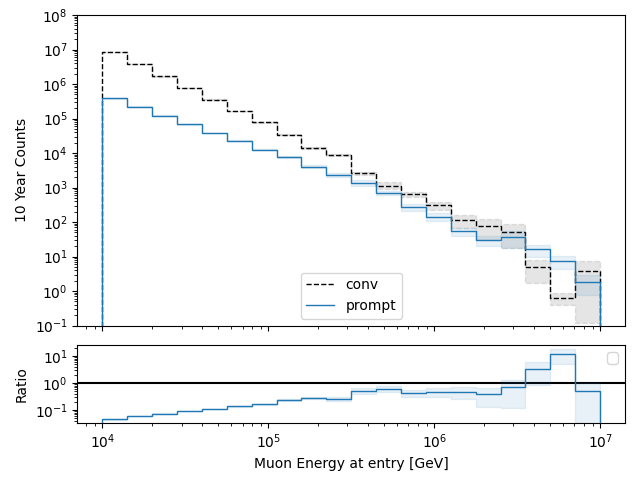
\includegraphics[width=0.4\textwidth]{Plots/spectrum_3_zenith_20ebins}
	\end{figure}
    \begin{itemize}
        \item Fitting of high Number of parameters requires good resolution $\rightarrow$ more bins
        \item Tests show extremely high significance
        \item What about the uncertainties?  
    \end{itemize}
\end{frame}
%\begin{frame}
%	\frametitle{What about the MC-uncertainties?}
%	\begin{itemize}
%		\item Good discovery-potential with systematics
%		\item Poisson Likelihood: MC assumed to be perfect estimate
%		\item Alternative: The SAY-likelihood
%	\end{itemize}
%\end{frame}
\begin{frame}
	\frametitle{The SAY-likelihood}
	\begin{itemize}
		\item Poisson likelihood:
        \begin{equation}
            L(\vec{\Theta}|k)=\frac{\lambda(\vec{\Theta})^ke^{-\lambda(\vec{\Theta})}}{k!}
        \end{equation}
        \item Assumption: Expectation exactly known
        \item For a limited number of sampled MC events this assumption is unrealistic
        \item Better: Consider distribution of weights based on MC truth:
        \begin{equation}
            L(\vec{\Theta}|k)=\int_0^{\inf}\frac{\lambda^ke^{-\lambda}}{k!}P(\lambda|\vec{w}(\vec{\Theta}))d\lambda
        \end{equation}
        \item This leads to:
        \begin{equation}
            L_{Eff}(\vec{\Theta}|k)=(\frac{\mu}{\sigma^2})^{\frac{\mu^2}{\sigma^2}+1}\Gamma(k+\frac{\mu^2}{\sigma^2}+1)(k!(1+\frac{\mu}{\sigma^2})^{k+\frac{\mu^2}{\sigma^2}+1}\Gamma(\frac{\mu^2}{\sigma^2}+1))^{-1}
        \end{equation}
	\end{itemize}
\end{frame}
\begin{frame}
	\frametitle{SAY vs Poisson}
    \begin{figure}
	    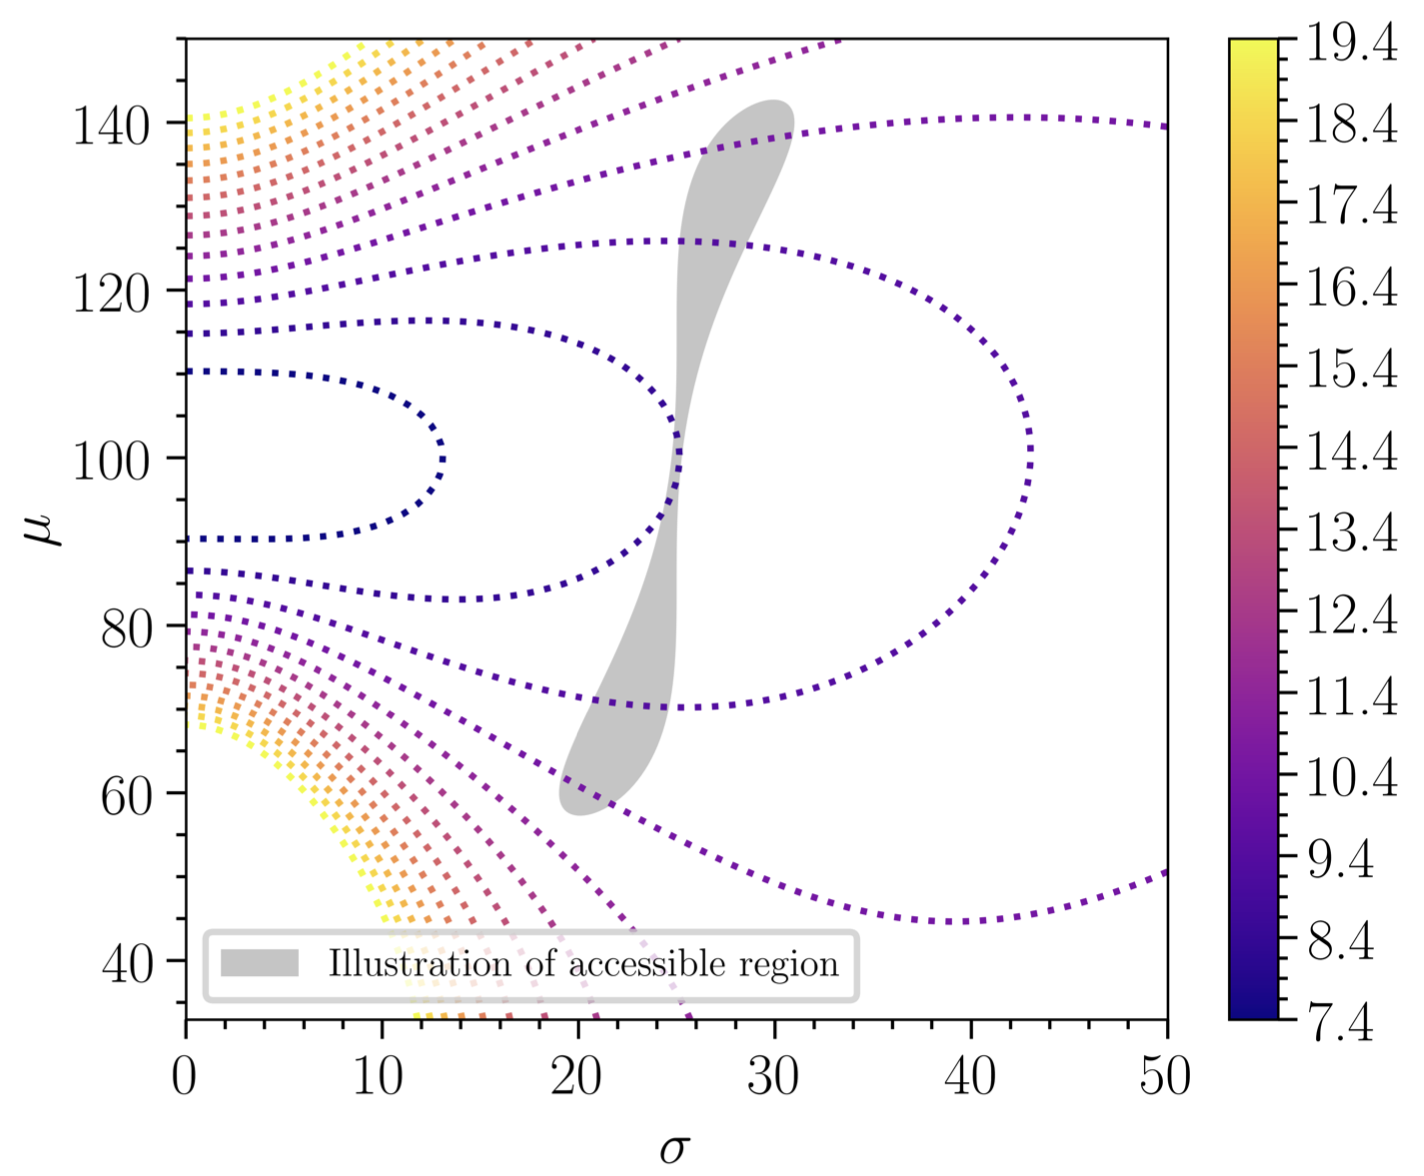
\includegraphics[width=0.35\textwidth]{Plots/SAY_paper}
        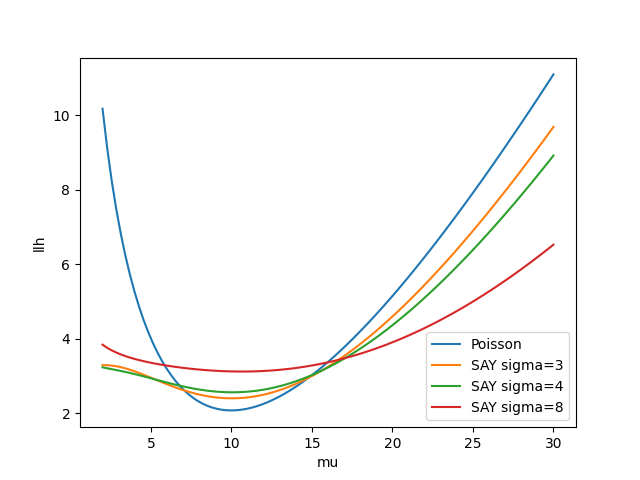
\includegraphics[width=0.35\textwidth]{Plots/SAY_visualization}
        \caption{Left: Contours of negative SAY log likelihood for $k=100$. Right: Poisson likelihood and SAY likelihood for $k=10$ for three different uncertainties}
    \end{figure}
    \begin{itemize}
        \item SAY likelihood is broader for higher uncertainties!
        \item Allows for konservative estimate when dealing with high MC-uncertainties
    \end{itemize}
\end{frame}
\begin{frame}
    \frametitle{SAY vs Poisson: Likelihood scan}
    \begin{figure}
        \centering
        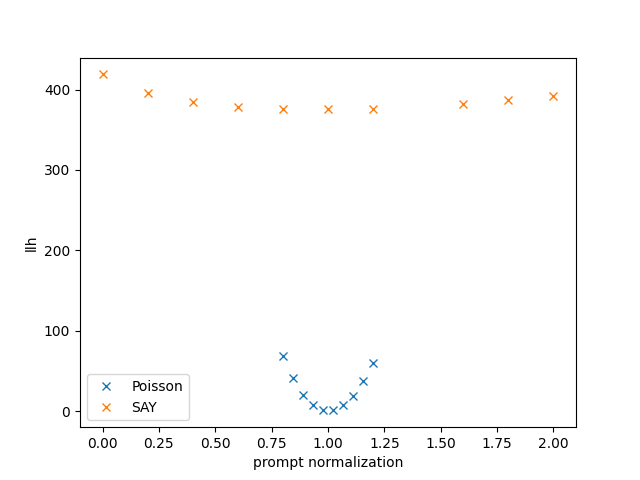
\includegraphics[width=0.5\textwidth]{Plots/prompt_norm_likelihoods}
        \caption{$1$D likelihood scans of the prompt component for both likelihoods}
    \end{figure}
    \begin{itemize}
        \item Likelihood scans reflect this: SAY likelihood has a much broader profile resulting in less significance
    \end{itemize}
\end{frame}
\begin{frame}
	\frametitle{Impact of SAY on the fit}
    \begin{minipage}{0.6\textwidth}
	    \begin{figure}
            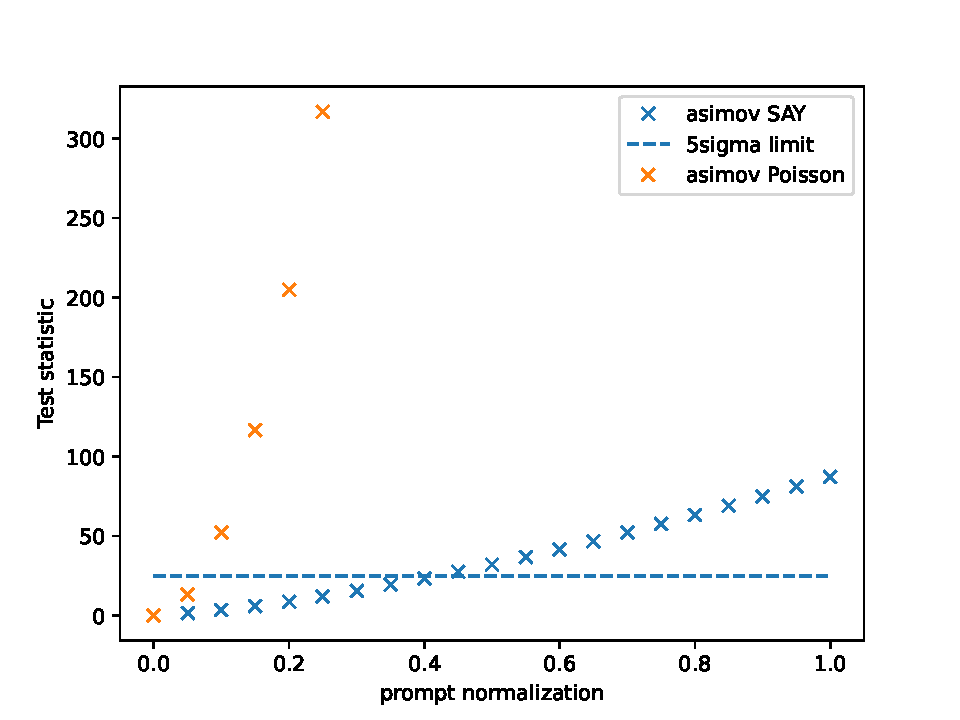
\includegraphics[width=\textwidth]{Plots/asimov_scan_say}
	    \end{figure}
    \end{minipage}
    \begin{minipage}{0.39\textwidth}
        \begin{itemize}
            \item SAY likelihood significantly reduces the discovery potential
            \item This reflects the high MC uncertainties in the high energy region
            \item SAY converges to Poisson for perfect MC statistic $\rightarrow$ no disadvantage in using it
        \end{itemize}
    \end{minipage}
\end{frame}
\begin{frame}
	\frametitle{Bias test and fit precision}
    \begin{minipage}{0.6\textwidth}
	    \begin{figure}
	    	\centering
            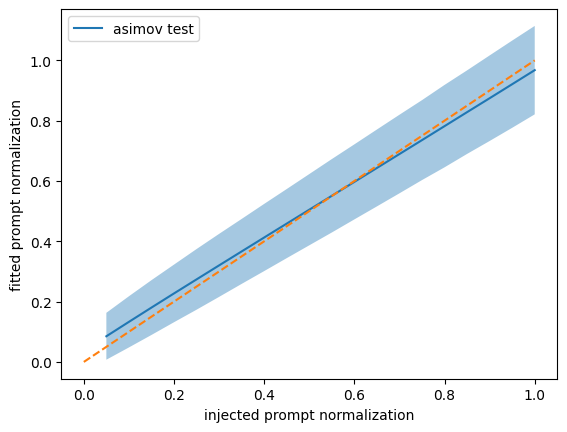
\includegraphics[width=0.5\textwidth]{Plots/asimov_bias_2.png}
            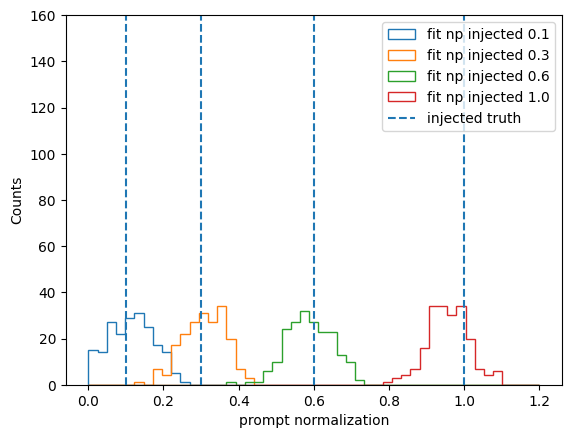
\includegraphics[width=0.5\textwidth]{Plots/Pseudoexperiment_fits}
	    \end{figure}
    \end{minipage}
    \begin{minipage}{0.39\textwidth}
        \begin{itemize}
            \item Bottom: Generated using Pseudoexperiments
            \item Top: Generated from asimov fit with uncertainty estimated by minimizer
            \item Unresolved bias!
        \end{itemize}
    \end{minipage}
\end{frame}
\begin{frame}
    \frametitle{Outlook}
    \begin{itemize}
        \item Include quality cuts (data level $5$) $\rightarrow$ Increase data-mc agreement
        \item Make control fit of conv in low energy region where you dont expect prompt events $\rightarrow$ Cross check for conventional fit 
        \item Try to test on Burnsample
        \item Problem: Low lifetime of a few months compared to ten years
        \item Include new Parameters:\begin{itemize}
            \item $n_{charmed}$,$n_{unflavoured}$: Contribution of charmed and unflavoured particles. Can these components be measured individually?
            \item $\Delta\gamma$: Potential shift in spectral indices of the components, softer or harder spectrum
            \item $\gamma_{CR}$: Cosmic ray gradient
            \item Use interpolation between primary models
        \end{itemize}
    \end{itemize}
\end{frame}
\begin{frame}
    \frametitle{Summary}
    \begin{minipage}{0.6\textwidth}
        \begin{figure}
            \centering
            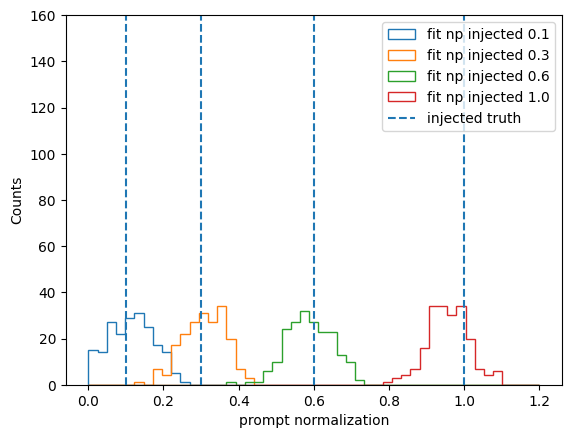
\includegraphics[width=0.5\textwidth]{Plots/Pseudoexperiment_fits}
            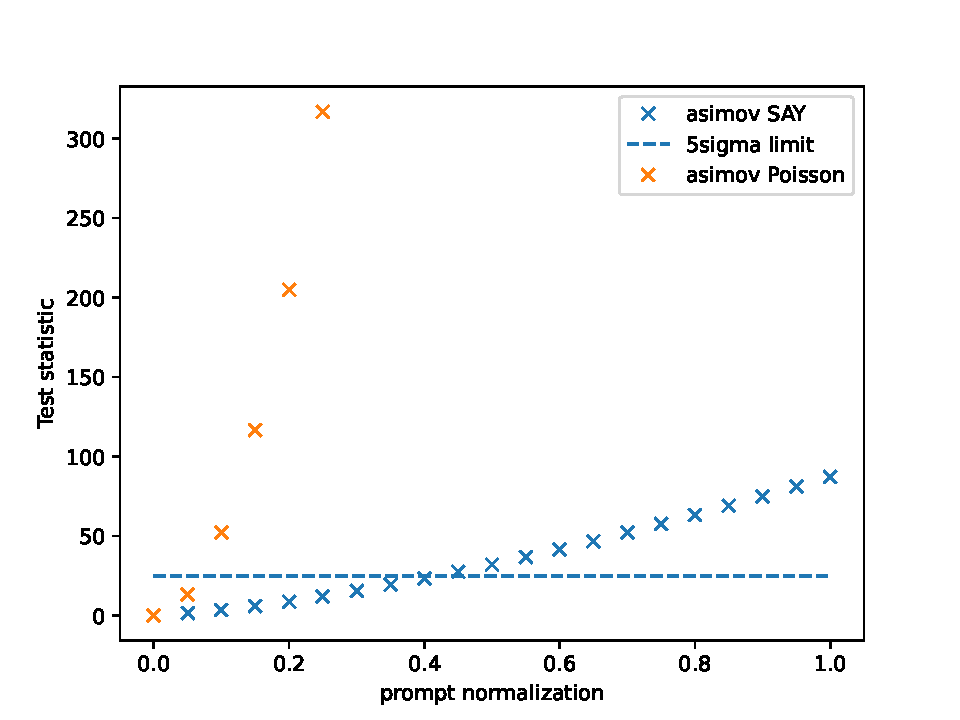
\includegraphics[width=0.5\textwidth]{Plots/asimov_scan_say}
        \end{figure}
    \end{minipage}
    \begin{minipage}{0.39\textwidth}
        \begin{itemize}
            \item Generate prompt tag in simulation
            \item Simulate up to high energies
            \item Use NNMFit to include systematics
            \item Estimate significance from
        \end{itemize}
    \end{minipage}
\end{frame}
\begin{frame}
    \frametitle{Backup: 2D histogram}
    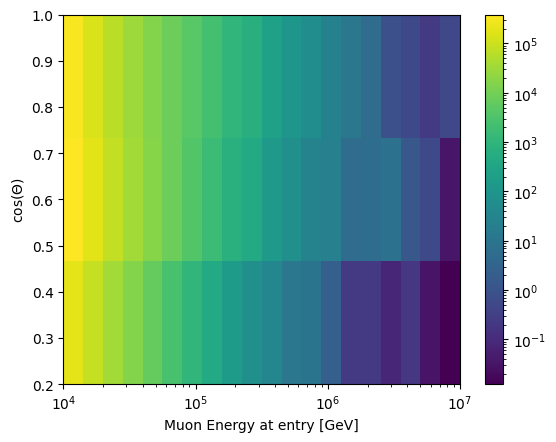
\includegraphics[width=0.6\textwidth]{Plots/2D_spectrum}
\end{frame}
%\begin{frame}
%\end{frame}
\end{document}
